\section{導入}

\subsection{計算可能解析}

計算可能解析 (Computable Analysis) \cite{weihrauch00:_comput_analy} では
計算可能性理論や計算量理論の視点から解析学を扱う. 
「計算可能な実数」や「多項式時間計算可能な実関数」といった概念を定義し, 
解析学に現れる様々な実数や実関数の本質的な難しさを分析する. 

離散的な対象においては「計算できる関数」はモデルによらず,
すべてチューリング機械で計算できるものと同値であることが知られているが,
実数計算においては, 計算できる関数が互いに異なる, いくつかのモデルが提唱されている.
本稿では,
「機械が実関数を計算する」ことを次のように定義する.

実関数 $f \colon \R \to \R$ を計算するといっても,
実数は有限の文字列で表されないため,
機械がその完全な値を読み書きすることはできない.
そこで実数を近似値の列で表現する.
有理数の列 $(r_n)_n$ が $x$ を表現するとは,
$(r_n)_n$ が $x$ へ速く収束すること, 
すなわち $|r_n - x| \le 2^{-n}$ を満たすこととする.
数列は $n \in \N$ を $r_n \in \Q$ へ移す関数と考えることもでき,
そのような関数または数列を実数の名と呼ぶ.

実関数を計算するモデルとしては神託チューリング機械を用いる. 
ある機械が関数 $f \colon [0, 1] \to \R$ を計算するとは,
入力となる実数 $x$ の名を神託として与えられ,
求める精度 $n$ を入力として与えられたとき,
有理数 $s_n$ で $|s_n - f(x)| \le 2^{-n}$ を満たすものを出力することとする.
この神託機械の資源を制限することで, 
実関数が多項式時間計算可能, 或いは多項式領域計算可能であることを
定義できる (\ref{section: preliminaries}節).

\subsection{問題と関連研究}

連続実関数 $g \colon [0,1] \times \R \to \R$ にたいして次の常微分方程式を考える. 
\begin{align}
 \label{eq:ode}
 h(0) & = 0, &
 h'(t) & = g(t,h(t)) \quad (t \in [0,1])
\end{align}
本稿では $g$ が多項式時間計算可能であるとき, 
解 $h$ がどれほど複雑でありうるかを考える.

$g$ に他に何の制限も設けない場合, 解 $h$ (一般に一意でない) は計算不能たりうるため,
様々な制限のもと $h$ の計算量が研究されている (表 \ref{table:related}).
この表では下に向うにつれて左列の条件が強まっている. 
Lipschitz 条件とは解 $h$ が一意であるための十分条件であり, 
これが満たされるときには, 解 $h$ は多項式領域計算可能であり, 
$\PSPACE$ 困難 (\ref{section: preliminaries}節で定義) でありうることがわかっている. 
つまり上界と下界が一致しているといえる (詳しくは河村 \cite{kawamura2010lipschitz}).
一方で $g$ が解析的であるとき, 解 $h$ も解析的となり, 
このとき $h$ は多項式時間計算可能である.

\begin{table}
\renewcommand\arraystretch{1.5}
\begin{center}
 \caption{多項式時間計算可能関数 $g$ の常微分方程式 (\ref{eq:ode}) の解 $h$ の計算量}
 \label{table:related}
 \begin{tabular}{lll}
  制限 & 上界 & 下界 \\
  \hline
   --- & --- & 計算不可能たりうる \cite{pour1979computable} \\
  $h$ が $g$ の唯一解 & 計算可能 \cite{coddington1955theory}
  & 任意の時間がかかりうる \cite{ko1983computational, miller1970recursive} \\
  $g$ が Lipschitz 条件を満たす & 多項式領域計算可能
      &	\PSPACE 困難になりうる \cite{kawamura2010lipschitz}\\
  $g$ が $(0, 1)$ 回連続微分可能 & 多項式領域計算可能 & \parbox[t]{14zw}{\PSPACE 困難になりうる\\{}[本稿定理\ref{DifferentiableIsPspace}]} \\
  $g$ が $(0, k)$ 回連続微分可能 & 多項式領域計算可能 & \parbox[t]{14zw}{\DIVPlog 困難たりうる\\{}[本稿定理\ref{KTimesIsPspace}]} \\
  $g$ が解析的 
  & 多項式時間計算可能 \cite{ko1988computing, kawamura2010complexity} 
  & ---
 \end{tabular}
\end{center}
\end{table}

そこで本稿ではこの隔たりを埋めるため, 滑らかな関数, 
つまり微分可能な $g$ について $h$ の計算量がどれほどになりうるかを調べ,
以下の結果を得た.

 \begin{theorem}
  \label{DifferentiableIsPspace}
  多項式時間計算可能かつ $(\infty, 1)$ 回連続的微分可能な
  実関数 $g \colon [0,1] \times [-1,1] \to \R$ であって, 
  常微分方程式(\ref{eq:ode})が
  $\PSPACE$ 困難な解 $h \colon [0, 1] \to \R$ をもつものが存在する.
 \end{theorem}

 \begin{theorem}
  \label{KTimesIsPspace}
  任意の自然数 $k \ge 2$ にたいして, 
  多項式時間計算可能かつ $(\infty, k)$ 回連続的微分可能な
  実関数 $g \colon [0,1] \times [-1,1] \to \R$ であって, 
  常微分方程式(\ref{eq:ode})が
  $\DIVPlog$ 困難な解 $h \colon [0, 1] \to \R$ をもつものが存在する.
 \end{theorem}

ここで $g \colon [0,1] \times \R \to \R$ でなく
$g \colon [0,1] \times [-1, 1] \to \R$ と書いたのは, 
本稿では実関数の多項式時間計算可能性を, 
定義域が有界閉領域のときにのみ定義するからである. 
このため $h$ が区間 $[-1, 1]$ の外に値を取ることがあると
方程式(\ref{eq:ode})が意味をなさなくなるが, 
定理\ref{DifferentiableIsPspace}, \ref{KTimesIsPspace}において $h$ が
解であるというのは, 
任意の $t \in [0, 1]$ について $h (t) \in [-1, 1]$ が満たされることも含めて述べている.
なお両定理とも Lipschitz 条件よりも強い仮定を置いているため, 
そのような $h$ は $g$ に対して, 存在すれば唯一である. 

 $\DIVPlog$ とは本稿 \ref{section: preliminaries} 節で定義する計算量クラスであり,
 $\DIVPlog \subseteq \PSPACE$ であるが, $\DIVPlog = \PSPACE$ か否かは
 わからない. 

 二変数関数 $g$ が $(i, j)$ 階連続微分可能であるとは,
 第一変数について $i$ 回, 第二変数について $j$ 回微分可能であり,
 その導関数が連続であることと定義する.
 この定義は一般的な多変数関数における $k$ 階連続的微分可能の定義
 (任意の $k$ 階導関数が存在し, それらがすべて連続)とは異なる.
 $(i,j)$ 回連続微分可能であれば $\min \{i, j\}$ 回連続微分可能であるため,
 定理 \ref{DifferentiableIsPspace}, \ref{KTimesIsPspace} は
 それぞれ $1$ 回連続微分可能, $k$ 回連続微分可能と置き換えても成り立つ.

 また定理 \ref{KTimesIsPspace} において
 任意の $k$ に対して $(\infty, k)$ 階微分可能な関数を考えているが,
 一つの関数が任意の $k$ にたいして $k$ 階微分であることを求めているわけではない.
 つまり $g$ が無限回微分可能であると制限しているわけではない. 
 無限回微分可能な関数に対する常微分方程式の計算量は今後の課題である.





\subsection{差分方程式}
\label{section:divp}

定理 \ref{DifferentiableIsPspace} と定理 \ref{KTimesIsPspace} の証明では,
まず滑らかな実関数の常微分方程式によって
ある種の「離散版」常微分方程式を模倣できることを示し, 
その離散版の方程式が$\PSPACE$困難ないし$\DIVPlog$困難であることを示す.
この節ではその離散版の方程式である「差分方程式」を定義する.

$[n] = \{0, \dots , n-1\}$ と書く.
関数 $G \colon [P] \times [Q] \times [R] \to \{-1, 0, 1\}$ にたいして,
関数 $H \colon [P + 1] \times [Q+1] \to [R]$ が
任意の $i \in [P],\ T \in [Q]$ について以下を満たすとき,
$H$ を $G$ の差分方程式の解と呼ぶ.
\begin{gather}
   H(i, 0) = H(0, T) = 0 
\\
   H(i + 1, T + 1) = H(i+1, T) + G(i, T, H(i, T))  \label{eq:divp}
\end{gather}
$P, Q, R$ をそれぞれ行数, 列数, 欄の大きさと呼ぶ.
$G$ と $H$ が常微分方程式の $g$ と $h$ に対応し,
$H(i, 0) = 0$ と言う条件が $h(0) = 0$,
式 (\ref{eq:divp}) と同値である $H(i + 1, T + 1) - H(i+1, T) = G(i, T, H(i, T))$
と言う条件が $h'(t) = g(t, h(t))$ と対応する.

以下では文字列 $u$ ごとに差分方程式 $G _u$ を一つ定めた族 $(G _u) _u$ を考える. 
 言語 $L$ がこの族 $(G_u)_u$ によって認識されるとは,
 各 $u$ にたいして $G_u$ の段数と列数, 解をそれぞれ $P_u, Q_u, H_u$ としたとき,
 $H_u(P_u, Q_u) = L(u)$ をみたすこととする[表 \ref{fig:divp}].
ここで言語 $L \subseteq \{0, 1\} ^*$ は
関数 $L \colon \{0, 1\} ^* \to \{0, 1\}$ と同一視し, 
$u \in L$ のとき $L (u) = 1$ としている. 

 \begin{figure}
  \label{fig:divp}
  \begin{center}
   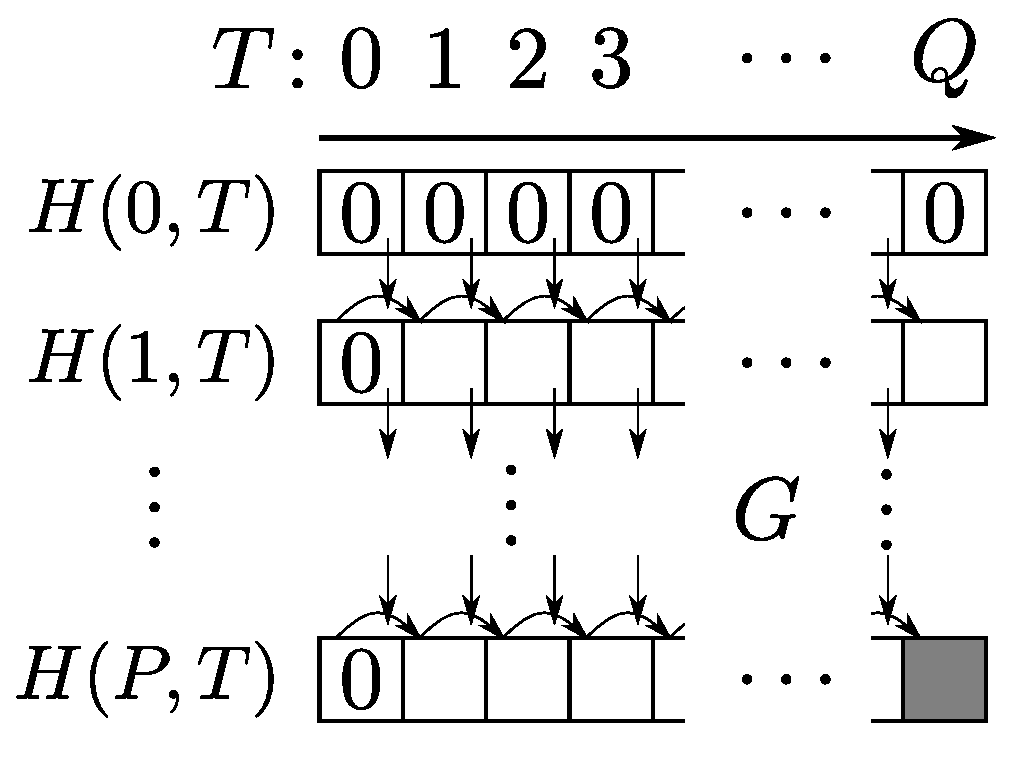
\includegraphics[height=0.2\textheight]{image/divp.eps}
  \end{center}
  \caption{差分方程式と認識される言語}
 \end{figure}

$(G_u)_u$ が{\bf 一様}であるとは,
各 $u$ について $G _u$ の段数, 列数及び欄の大きさが $|u|$ の多項式の指数($2^{\mathrm{poly} (|u|)}$)で抑えられ, 
かつ与えられた $(u, i, T, Y)$ から多項式時間で $G_u(i, T, Y)$ が
計算できることと定義する.

$G_u$ の段数がさらに $|u|$ の多項式, 対数で抑えられるとき, 
族 $(G_u) _u$ はそれぞれ\emph{多項式段}, \emph{対数段}であるという. 
多項式段, 対数段の一様関数族によって認識される言語のクラスを
それぞれ $\DIVPpoly$, $\DIVPlog$ と名づける.
この記法を使うと
河村の論文では次が示されている.

 \begin{lemma}[補題 4.7. \cite{kawamura2010lipschitz}]
  \label{WeakFeedback}
  $\DIVPpoly = \PSPACE$.
 \end{lemma}

 $\DIVPlog \subseteq \DIVPpoly = \PSPACE$ であるが, 
 $\DIVPlog = \PSPACE$ か否かは未解決である.
 また \DIVPlog の計算量の下限として $\sharp${\bf P} が考えられる.
 \DIVPlog が決定問題であるのに対し, $\sharp${\bf P} は関数問題であるため
 単純には比較できない.
 そこで一様な $(G_u)_u$ の2段の差分方程式によって定義される関数問題のクラスを考える.
 最後の欄の値は $H_u(1, Q_u) = \sum_{t < Q_u} G_u(0, t, 0)$.
 $u$ について多項式時間関数 $G_u(0, t, 0)$ の和になっているため,
 差分方程式の関数問題クラスは数え上げ問題である $\sharp${\bf P} を含む.
